% Fig 4 - B1 fairness protocol.
%
% Three encoders side-by-side (JEPA, Fukami AE, POD) feed into ONE identical
% unified transformer predictor. The predictor rolls out latent trajectories,
% which are mapped to physical observables (C_L, I_y, wake_enstrophy) by a
% shared probe head. Loss is L_pred on the rolled-out latents; final eval is
% the Markov closure R^2 of each observable.
%
% Standalone-compilable: pdflatex fig4_b1_fairness.tex

\documentclass[border=10pt,tikz]{standalone}
\usepackage{tikz}
\usepackage{amsmath,amssymb}
\usetikzlibrary{positioning,arrows.meta,fit,shapes.geometric,calc,backgrounds}

\begin{document}

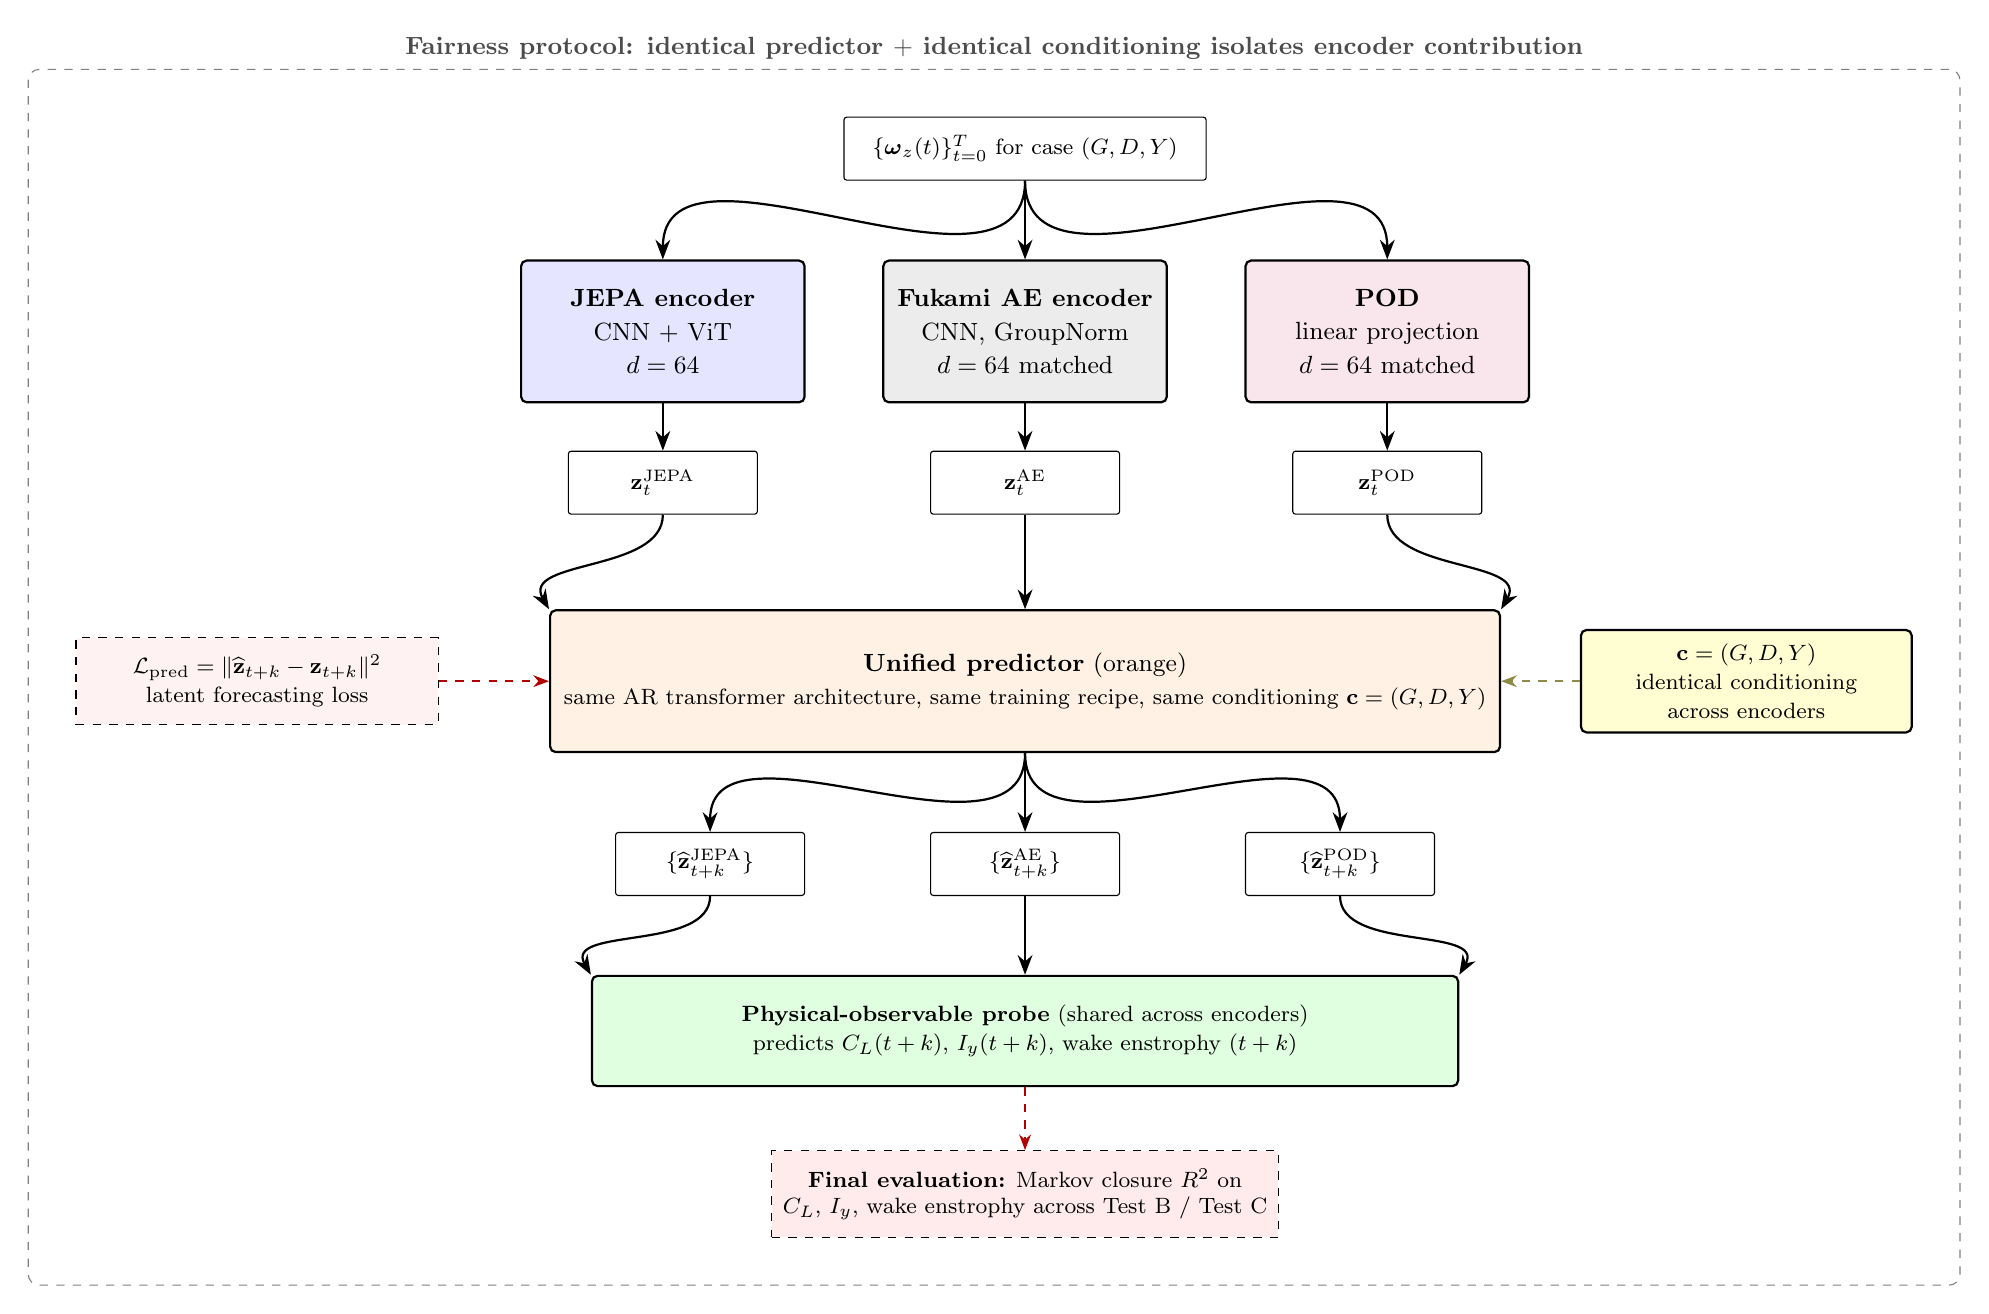
\begin{tikzpicture}[
    font=\small,
    box/.style={draw, rounded corners=2pt, align=center, inner sep=5pt, thick},
    encjepa/.style={box, fill=blue!10, minimum width=36mm, minimum height=18mm},
    encfukami/.style={box, fill=gray!15, minimum width=36mm, minimum height=18mm},
    encpod/.style={box, fill=purple!10, minimum width=36mm, minimum height=18mm},
    predictor/.style={box, fill=orange!10, minimum width=110mm, minimum height=18mm,
                      thick},
    probe/.style={box, fill=green!12, minimum width=110mm, minimum height=14mm,
                  font=\footnotesize},
    state/.style={draw, rectangle, rounded corners=1pt, fill=white,
                  minimum height=8mm, minimum width=24mm, inner sep=2pt,
                  font=\footnotesize},
    cond/.style={box, fill=yellow!18, minimum width=42mm, minimum height=12mm,
                 font=\footnotesize},
    loss/.style={draw, rectangle, dashed, fill=red!5, inner sep=4pt,
                 minimum height=11mm, minimum width=46mm, align=center,
                 font=\footnotesize},
    note/.style={align=center, font=\footnotesize\itshape},
    arr/.style={-{Stealth[length=2.5mm]}, thick},
    arrshort/.style={-{Stealth[length=2mm]}, semithick},
    lossarr/.style={-{Stealth[length=2mm]}, dashed, semithick, red!70!black},
    arrcond/.style={-{Stealth[length=2mm]}, semithick, yellow!50!black, dashed}
  ]

  % ========= shared input (per-case omega trajectory) =========
  \node[state, minimum width=46mm] (input)
    {$\{\boldsymbol{\omega}_z(t)\}_{t=0}^{T}$ for case $(G, D, Y)$};

  % ========= three encoders side by side =========
  \node[encjepa,   below=10mm of input, xshift=-46mm] (ejepa)
    {\textbf{JEPA encoder} \\[1pt]
     CNN $+$ ViT \\[1pt]
     $d = 64$};
  \node[encfukami, below=10mm of input]              (efuk)
    {\textbf{Fukami AE encoder} \\[1pt]
     CNN, GroupNorm \\[1pt]
     $d = 64$ matched};
  \node[encpod,    below=10mm of input, xshift=46mm] (epod)
    {\textbf{POD} \\[1pt]
     linear projection \\[1pt]
     $d = 64$ matched};

  \draw[arr] (input.south) to[out=-90,in=90] (ejepa.north);
  \draw[arr] (input.south) to[out=-90,in=90] (efuk.north);
  \draw[arr] (input.south) to[out=-90,in=90] (epod.north);

  % ========= per-encoder latent stream =========
  \node[state, below=6mm of ejepa] (zjepa)
    {$\mathbf{z}^{\text{JEPA}}_{t}$};
  \node[state, below=6mm of efuk]  (zfuk)
    {$\mathbf{z}^{\text{AE}}_{t}$};
  \node[state, below=6mm of epod]  (zpod)
    {$\mathbf{z}^{\text{POD}}_{t}$};

  \draw[arr] (ejepa) -- (zjepa);
  \draw[arr] (efuk)  -- (zfuk);
  \draw[arr] (epod)  -- (zpod);

  % ========= unified predictor =========
  \node[predictor, below=12mm of zfuk] (pred)
    {\textbf{Unified predictor} (orange) \\[1pt]
     \footnotesize same AR transformer architecture, same training recipe, same conditioning $\mathbf{c}=(G,D,Y)$};

  \draw[arr] (zjepa.south) to[out=-90,in=120] (pred.north west);
  \draw[arr] (zfuk.south)  -- (pred.north);
  \draw[arr] (zpod.south)  to[out=-90,in=60]  (pred.north east);

  % conditioning c enters the predictor from the right
  \node[cond, right=10mm of pred] (cond)
    {$\mathbf{c} = (G, D, Y)$ \\[1pt]
     identical conditioning \\[1pt] across encoders};
  \draw[arrcond] (cond.west) -- (pred.east);

  % ========= rolled-out latent streams =========
  \node[state, below=10mm of pred, xshift=-40mm] (rolljepa)
    {$\{\widehat{\mathbf{z}}^{\text{JEPA}}_{t+k}\}$};
  \node[state, below=10mm of pred]               (rollfuk)
    {$\{\widehat{\mathbf{z}}^{\text{AE}}_{t+k}\}$};
  \node[state, below=10mm of pred, xshift=40mm]  (rollpod)
    {$\{\widehat{\mathbf{z}}^{\text{POD}}_{t+k}\}$};

  \draw[arr] (pred.south) to[out=-90,in=90] (rolljepa.north);
  \draw[arr] (pred.south) to[out=-90,in=90] (rollfuk.north);
  \draw[arr] (pred.south) to[out=-90,in=90] (rollpod.north);

  % ========= L_pred loss on rolled-out latents (left side) =========
  \node[loss, left=14mm of pred] (lpred)
    {$\mathcal{L}_{\text{pred}} = \| \widehat{\mathbf{z}}_{t+k} - \mathbf{z}_{t+k} \|^{2}$ \\[1pt]
     latent forecasting loss};
  \draw[lossarr] (lpred.east) -- (pred.west);

  % ========= shared probe to physical observables =========
  \node[probe, below=10mm of rollfuk] (probe)
    {\textbf{Physical-observable probe} (shared across encoders) \\[1pt]
     predicts $C_L(t+k)$, $I_y(t+k)$, wake enstrophy $(t+k)$};

  \draw[arr] (rolljepa.south) to[out=-90,in=120] (probe.north west);
  \draw[arr] (rollfuk.south)  -- (probe.north);
  \draw[arr] (rollpod.south)  to[out=-90,in=60]  (probe.north east);

  % ========= final eval =========
  \node[loss, below=8mm of probe, fill=red!8] (eval)
    {\textbf{Final evaluation:} Markov closure $R^2$ on \\
     $C_L$, $I_y$, wake enstrophy across Test B / Test C};
  \draw[lossarr] (probe.south) -- (eval.north);

  % ========= background frame =========
  \begin{scope}[on background layer]
    \node[draw=black!50, rounded corners=4pt, dashed, inner sep=6mm,
          fit=(input)(ejepa)(efuk)(epod)(zjepa)(zfuk)(zpod)(pred)(cond)(lpred)
              (rolljepa)(rollfuk)(rollpod)(probe)(eval),
          label={[black!70,font=\small\bfseries]above:%
            Fairness protocol: identical predictor $+$ identical conditioning isolates encoder contribution}] {};
  \end{scope}

\end{tikzpicture}

\end{document}
